\section{问题重述与建模思路}

\subsection{题目任务}

2023 年 6 月，“泰坦号”潜水器在北大西洋 3800 m 深处失事后，国际社会开始重视
小型旅游潜水器的搜救能力建设。2024 年 MCM 问题 B 要求以一艘可载 6 人、额定潜深
1000 m 的旅游潜水器为对象，完成四项任务：

\begin{enumerate}[leftmargin=1.8em,itemsep=0pt]
\item \textbf{Locate（定位）}：建立潜水器失联后位置随时间变化的模型，量化位置不确定性；
\item \textbf{Search（搜索）}：建立搜索模型，给出发现概率随时间的变化；
\item \textbf{Prepare（装备）}：为运营公司推荐搜索装备配置，权衡时间、成功率与成本；
\item \textbf{Extrapolate（外推）}：将模型推广到其他海域及其他潜水器情形。
\end{enumerate}

题目给定的场景是：潜水器在伊奥尼亚海一处小岛（Moni Strofadon，约
$37.249^\circ$N、$21.014^\circ$E）附近搭载游客下潜后失联；母船在失事点上空。

\subsection{三个关键判断}

\paragraph{判断一：这是“搜索问题”，不是“轨迹预测问题”。}
定位模型的价值不在于给出唯一位置，而在于给出\emph{位置的概率分布及其随时间的增长}；
搜救装备与策略要针对这个分布做贝叶斯更新。因此我们把定位模型输出为集合预报
（30\,000 条轨迹），直接作为搜索模型的先验。

\paragraph{判断二：搜救开始时位置并非完全未知。}
题目要求我们假设：每次搜救时，搜救方知道目标在“水平半径 100 m、垂直 $\pm$10 m 的
圆柱”内。真正的不确定性来自\emph{失联之后}的漂移与失效模式分支。这一设定把问题
从“大海捞针”变为“从一个小圆柱出发、跟着预测云走”的追踪搜索，
也解释了下文为什么“漂移绝对距离大”不一定意味着“更难搜”。

\paragraph{判断三：决策变量是“装备组合 + 响应时间”，而不是单一装备。}
题目要求推荐装备，而装备的价值取决于它覆盖哪一类目标（水面、水柱、海底）。
因此我们建立“装备能力矩阵 $\times$ 目标类别”的探测模型，并用统一的时间–成功率–成本
指标比较 7 种单船组合与 15 种多船/多 AUV 组合。

\subsection{分层架构}

模型分为三层（\figref{fig:framework}），层间只通过“初始位置集成”与“轨迹数据”通信，
因此任一层的修改都不会破坏其他层：

\begin{enumerate}[leftmargin=1.8em,itemsep=0pt]
\item \textbf{上层}：给定初始位置分布（4$\times$4 km 均匀 $\times$ 深度指数分布）
      与搜救知识圆柱（$r=100$ m，$\Delta z=\pm10$ m）；
\item \textbf{定位层}：失效树 + 垂向动力学 + 四维流场 + 海底滑移，生成 30\,000 条轨迹；
\item \textbf{搜索/装备层}：声呐探测模型 + 滚动规划 + 贝叶斯更新，评估
      7 种单船组合与 15 种协同组合。
\end{enumerate}

\begin{figure}[H]
\centering
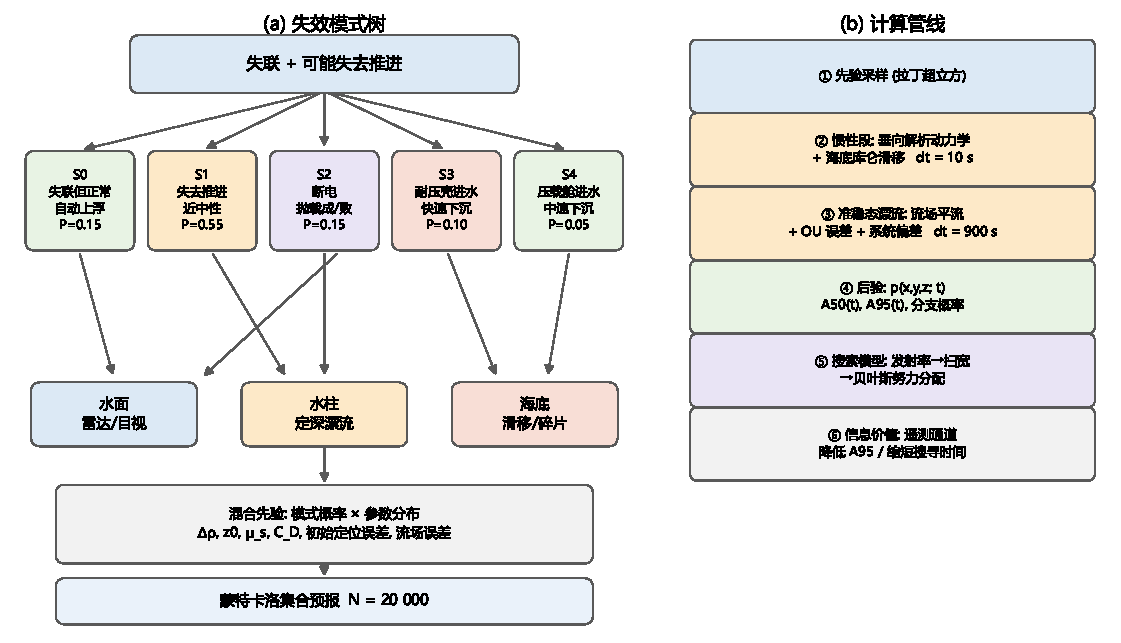
\includegraphics[width=0.86\textwidth]{fig_p2_framework}
\caption{三层模型框架：上层给定初始位置，中层是失效树驱动的集合预报，
下层是搜索与装备决策。层间通过标准化的“初始位置表”和“轨迹集”通信。}
\label{fig:framework}
\end{figure}

\subsection{本文贡献}

\begin{enumerate}[leftmargin=1.8em,itemsep=0pt]
\item 建立了含 5 种失效模式、浮力异常、四维流场、海底接触与滑移的潜水器集合预报模型，
      并用解析解、方差检验、阈值检验做了\textbf{可复现的验证}；
\item 建立了“声呐扫宽–目标类别–深度能力”探测模型与逐小时滚动规划算法，
      给出 7 种装备组合的完整时间–成功率–成本曲线；
\item 建立了多船/多 AUV 的协同搜索模型（小时内认领 + 重复扫描惩罚），
      证明“先加船、后加 AUV”的边际效益规律；
\item 在两个海域（伊奥尼亚海、加勒比海）上验证模型的可迁移性，并明确指出
      “完美预报假设”对强流海域结论的影响方向。
\end{enumerate}
